\pdfminorversion=4
\documentclass{beamer}
\usepackage[ngerman]{babel}
\usepackage[utf8]{inputenc}
\usepackage{graphicx}
\usetheme{Warsaw}

\title{Mit Kryptographie die Welt retten}
\subtitle{Cypherpunk in Theorie und Praxis}
\author{Sebastian Beschke \\ \texttt{sebastian@sbeschke.de}}
\institute{Chaostreff Tübingen}
\date{01. 10. 2011}
\begin{document}

\AtBeginSection[]
{
	\begin{frame}
		\begin{center}
		\Large{\insertsection}
		\end{center}
	\end{frame}
}

\begin{frame}
\titlepage
\end{frame}


\begin{frame}
	\frametitle{Überblick}
	\tableofcontents
\end{frame}

\section{Einführung in die Kryptographie}

\begin{frame}
\frametitle{Eine einfache Chiffre}
\begin{columns}

\column{0.5\textwidth}
	\texttt{FBSKHUSXQNV ZULWH FRGH}

\pause	\texttt{cypherpunks write code}

\column{0.5\textwidth}
\pause	\(K=3\)

	\textit{Schlüssel}

\end{columns}
\end{frame}

\begin{frame}
\frametitle{Symmetrische und Public-Key-Verschlüsselung}
\begin{columns}

\column{0.5\textwidth}
	\textbf{Symmetrisches Verfahren:}
	
	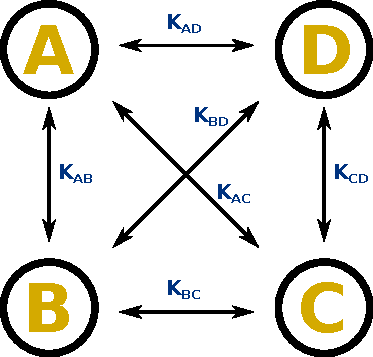
\includegraphics[width=0.9\textwidth]{images/symmetric.pdf}\\

	\(\Rightarrow \frac{n(n-1)}{2}\) Schlüssel

\pause
\column{0.5\textwidth}
	\textbf{Public-Key-Verfahren:}

	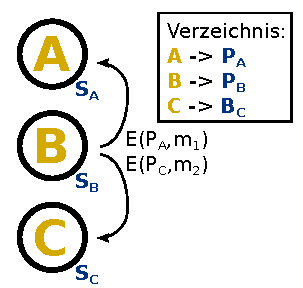
\includegraphics[width=0.9\textwidth]{images/asymmetric2.pdf}\\

	\(\Rightarrow 2n\) Schlüssel

\end{columns}
\end{frame}

\begin{frame}
\frametitle{Hybride Verfahren}

\begin{itemize}
	\item Public-Key-Kryptographie ist aufwändig zu berechnen
	\item Daher oft hybrider Ansatz:
	\begin{itemize}
		\item Austausch eines Schlüssels mittels Public-Key-Kryptographie
		\item Anschließend symmetrische Verschlüsselung mit diesem Schlüssel
		\item Der Schlüssel ist dann in der Regel kurzlebig
	\end{itemize}
\end{itemize}
\end{frame}

\begin{frame}
\frametitle{Das RSA-Verfahren}

	\begin{itemize}
		\item RSA ist eines der ältesten Public-Key-Verfahren (1978)
		\item Auch heute noch ein Standard-Verfahren
		\item Basiert auf der Modulo-Rechnung und dem Satz von Euler
		\item Deshalb jetzt ein wenig Mathe\dots
	\end{itemize}
\end{frame}

\begin{frame}
\frametitle{Modulo-Rechnung}
	\begin{itemize}
		\item Modulo-Rechnung ist das Rechnen mit Resten
		\item \(4 \cdot 4 \equiv \ ?\ (\text{mod}\ 5) \)
\pause		\item \(4 \cdot 4 = 16\)
\pause		\item \(16 : 5 = 3 \text{ Rest } \textbf{1}\)
\pause		\item Also \(4 \cdot 4 \equiv 1\ (\text{mod}\ 5) \)
	\end{itemize}
\end{frame}


\begin{frame}
\frametitle{Der Satz von Euler}

\begin{itemize}
	\begin{definition}[Die Eulersche \(\varphi\)-Funktion]
		\(\varphi(n) = \) Anzahl der zu \(n\) teilerfremden Zahlen \(\leq n\)
	\end{definition}
\pause	\item Ist \(p\) eine Primzahl, so ist \(\varphi(p) = p-1\)
	\item Ist \(n=pq\), \(p,q\) prim, so ist \(\varphi(n) = (p-1)(q-1)\)

\pause	\begin{theorem}[Der Satz von Euler]
		Seien \(a\) und \(n\) teilerfremd.
		Dann gilt \(a^{\varphi(n)} \equiv 1 \ (\textnormal{mod}\ n)\)
	\end{theorem}
\end{itemize}
\end{frame}

\begin{frame}
\frametitle{Verschlüsseln mit dem Satz von Euler}

	\begin{theorem}[Der Satz von Euler]
		Seien \(a\) und \(n\) teilerfremd.
		Dann gilt \(a^{\varphi(n)} \equiv 1 \ (\textnormal{mod}\ n)\)
	\end{theorem}

	\begin{itemize}
		\item Sei \(n\) das Produkt zweier Primzahlen \(p,q\)
		\item Angenommen, wir haben \(e,d\) mit \(ed = k \cdot \varphi(n) + 1\)
\pause		\item Sei \(m\) eine Nachricht.
		\item \(c \equiv m^e \ (\text{mod}\ n)\) ist dann die verschlüsselte Nachricht.
\pause		\item Kennt man \(d\), kann man sie entschlüsseln: \(c^d \equiv m^{ed} \equiv m^{k \cdot \varphi(n) + 1} \equiv m \cdot m^{k \cdot \varphi(n)} \equiv m \ (\textnormal{mod}\ n)\)
	\end{itemize}
\end{frame}

\begin{frame}
\frametitle{RSA-Verschlüsselung}

	\begin{center}
	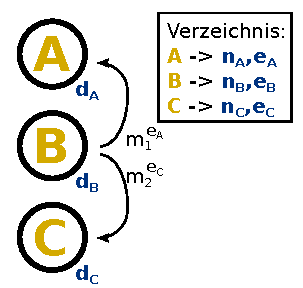
\includegraphics[height=0.8\textheight]{images/rsa.pdf}
	\end{center}
\end{frame}

\begin{frame}
\frametitle{Sicherheit von RSA}

\begin{itemize}
	\item Ein Angreifer könnte \(\log_e m^e\) berechnen.
	\begin{itemize}
	\item Das ist bei Modulorechnung sehr schwierig.
	\end{itemize}
\pause	\item Oder er könnte versuchen, \(d\) zu bestimmen.
	\begin{itemize}
	\item Der Knackpunkt: Zur Bestimmung von \(d\) braucht man \(\varphi(n)\)
	\item Leicht zu bestimmen, wenn man \(p,q\) kennt: \(\varphi(n)=(p-1)(q-1)\).
	\item Sonst aber sehr schwer zu bestimmen.
	\item[\(\Rightarrow\)] \(d\) zu bestimmen, ist so schwer, wie die Primfaktorzerlegung von \(n\).
	\end{itemize}
\end{itemize}
\end{frame}

\section{Privatsphäre unter Beschuss}

\begin{frame}
\frametitle{Die Rolle von Kryptographie}

\begin{itemize}
	\item Kryptographie: Metier von Geheimdiensten und Geheimniskrämern?
	\item Nicht im Informationszeitalter!
\end{itemize}
\begin{columns}

\column{0.5\textwidth}
	\begin{center}
	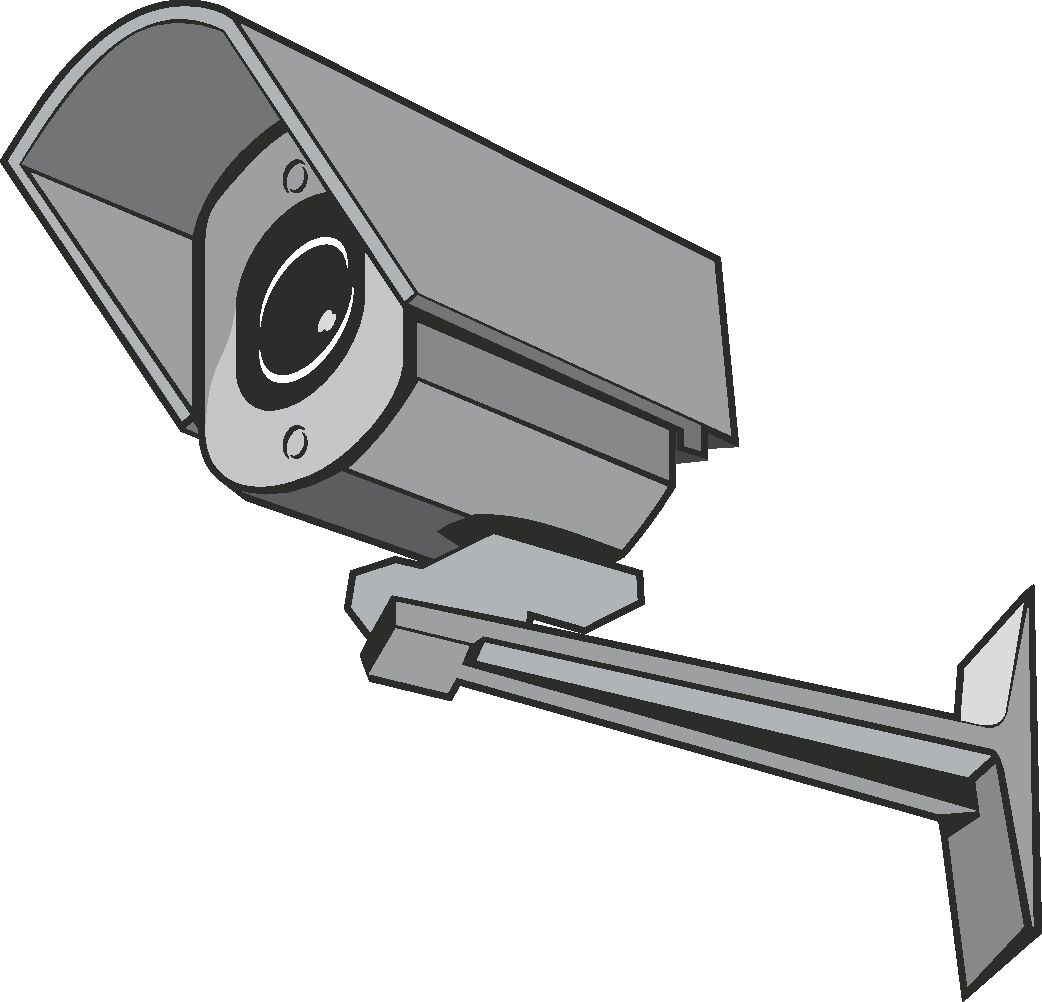
\includegraphics[height=0.4\textheight]{images/surveillancecamera.pdf}
	\end{center}

\column{0.5\textwidth}
	\begin{center}
	
\includegraphics[height=0.3\textheight]{images/fbgoogle.png}
	\end{center}

\end{columns}
\end{frame}

\begin{frame}
\frametitle{Was heißt eigentlich „Privatsphäre“?}
	
	\begin{itemize}
		\item Privatsphäre ist nicht nur Verschlüsselung:
		\begin{itemize}
			\item Anonymität
			\item Abstreitbarkeit
			\item Authentifizierung
		\end{itemize}
\pause		\item Privatsphäre ist nicht Geheimnistuerei:
		\begin{itemize}
			\item \textit{Geheime} Informationen soll \textit{niemand} erfahren
			\item \textit{Private} Informationen soll \textit{nicht jeder} erfahren
		\end{itemize}
	\end{itemize}

	\begin{quote}
		“Privacy is the power to selectively reveal oneself to the world.”\\
		\textnormal{Eric Hughes, A Cypherpunk’s Manifesto}
	\end{quote}

\end{frame}

\begin{frame}
\frametitle{Der Kampf um die Privatsphäre}

	\begin{itemize}
		\item Privatsphäre ist ein wiederkehrendes Thema der politischen Debatte in Deutschland:
		\begin{itemize}
			\item Klarnamenspflicht im Internet
			\item Vorratsdatenspeicherung
			\item Bundestrojaner
			\item Zensur(sula)gesetz
			\item Übermittlung von Fluggastdaten
			\item usw. usf.
		\end{itemize}

\pause		\item oder auch kürzlich:
	\end{itemize}
	\begin{quote}
		„Eine anonyme Teilhabe am politischen Meinungs- und Willensbildungsprozess ist abzulehnen.“\\
		\textnormal{Positionspapier der CDU/CSU-Fraktion im Bundestag zum Thema „Freiheit des Internet“}
	\end{quote}
\end{frame}

\begin{frame}
\frametitle{Diskrepanzen}

	\begin{itemize}
		\item In der „realen Welt“ ist Privatsphäre oft der Standard.
		\begin{itemize}
			\item Bargeld, Briefgeheimnis…
		\end{itemize}
	
		\ \\
	
		\item In der digitalen Welt sieht das meistens anders aus:
		\begin{itemize}
			\item Standardmäßig unverschlüsselte Übertragung von Webseiten, E-Mail, Chatnachrichten\dots
			\item Internet-Verbindungen sind über den Provider zurückverfolgbar
		\end{itemize}
	\end{itemize}
\end{frame}

\begin{frame}
\frametitle{Das \textit{Cypherpunk’s Manifesto}}

	\begin{itemize}
		\item Eine offene Gesellschaft braucht Privatsphäre
		\item Regierungen und Konzerne werden Privatsphäre nicht freiwillig schaffen
		\item Kryptographie ist das Mittel zur Wahrung der Privatsphäre
		\item Cypherpunks machen entsprechende Software
	\end{itemize}

	\begin{quote}
		“Cypherpunks write code.”
	\end{quote}
\end{frame}

\begin{frame}
\frametitle{Interessante Projekte}

	\begin{itemize}
		\item Bitcoin
		\item Freenet
		\item Off-the-Record messaging
		\item Tor
	\end{itemize}
\end{frame}

\section{Die Anonymisierungssoftware Tor}

\begin{frame}
\frametitle{Überblick über Tor}

\begin{itemize}
	\item Das Tor-Projekt…
	\begin{itemize}
		\item Entstanden als Weiterentwicklung des “Onion Routing”-Projekts des US Naval Research Laboratory
		\item Später finanziert durch die Electronic Frontier Foundation
		\item Seit 2006 ist das “Tor Project” eine Nonprofit-Organisation in den USA
	\end{itemize}

	\item Ziele von Tor
	\begin{itemize}
		\item Verschleiern: Wer kommuniziert mit wem?
		\item Umgehen von Zensurschranken
		\item Anonymes Bereitstellen von Informationen
	\end{itemize}
\end{itemize}
	
\end{frame}

\begin{frame}
\frametitle{Netzwerkstruktur von Tor}

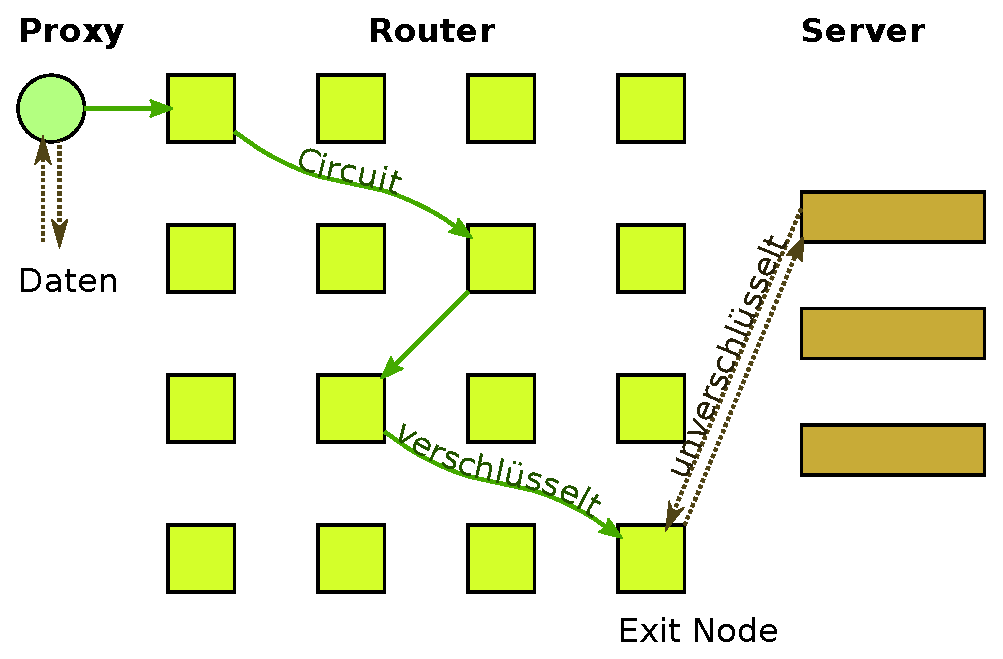
\includegraphics[width=\textwidth]{images/circuit.pdf}
\end{frame}

\begin{frame}
\frametitle{Aufbau eines Circuit}

\includegraphics<1>[width=\textwidth]{images/circuit_create.pdf}
\includegraphics<2>[width=\textwidth]{images/circuit_extend.pdf}
\end{frame}

\begin{frame}
\frametitle{Weiterleiten von Daten}

\includegraphics<1>[width=\textwidth]{images/circuit_relay.pdf}
\includegraphics<2>[width=\textwidth]{images/circuit_response.pdf}
\end{frame}

\begin{frame}
\frametitle{Anonymisierung}

\begin{itemize}
	\item Niemand erfährt, mit wem der Sender kommuniziert
	\begin{itemize}
		\item Der Server denkt, die Anfrage käme vom Exit Node
		\item Jeder Knoten im Circuit kennt nur seine Nachbarn
		\item Nur der Exit Node kann das Ziel des Datenpakets sehen
	\end{itemize}
	\item Aber:
	\begin{itemize}
		\item Der Exit Node sieht den Datenverkehr im Klartext
		\item Daher ist Ende-zu-Ende-Verschlüsselung zum Server sinnvoll
		\item Trotzdem kann das Datenpaket identifizierende Daten beinhalten
	\end{itemize}
\end{itemize}
\end{frame}

\section{Zusammenfassung}

\begin{frame}
\frametitle{Zusammenfassung}

\begin{itemize}
	\item Der Schutz der Privatsphäre ist wichtig
	\item Geschickter Einsatz von Kryptographie kann hierbei helfen
	\item Es ist schwer, ein wasserdichtes Kryptosystem zu bauen
	\item Selbst ein wasserdichtes System kann durch Fehler auf anderen Ebenen außer Kraft gesetzt werden
	\item Aber: Die Grundprinzipien sind einfach zu verstehen – Jede/r kann mitdenken
\end{itemize}
\end{frame}

\end{document}
